\documentclass[letterpaper,9pt,twoside,printwatermark=false]{pinp}

%% Some pieces required from the pandoc template
\providecommand{\tightlist}{%
  \setlength{\itemsep}{0pt}\setlength{\parskip}{0pt}}

% Use the lineno option to display guide line numbers if required.
% Note that the use of elements such as single-column equations
% may affect the guide line number alignment.

\usepackage[T1]{fontenc}
\usepackage[utf8]{inputenc}

% The geometry package layout settings need to be set here...
\geometry{layoutsize={0.95588\paperwidth,0.98864\paperheight},%
          layouthoffset=0.02206\paperwidth,%
		  layoutvoffset=0.00568\paperheight}

\definecolor{pinpblue}{HTML}{185FAF}  % imagecolorpicker on blue for new R logo
\definecolor{pnasbluetext}{RGB}{101,0,0} %



\title{DALITE Q7 - Two Sample Inference. Solutions.}

\author[a]{EPIB607 - Inferential Statistics}

  \affil[a]{Fall 2018, McGill University}

\setcounter{secnumdepth}{5}

% Please give the surname of the lead author for the running footer
\leadauthor{Bhatnagar and Hanley}

% Keywords are not mandatory, but authors are strongly encouraged to provide them. If provided, please include two to five keywords, separated by the pipe symbol, e.g:
 \keywords{  Two sample means |  Two sample proportions  }  

\begin{abstract}
This DALITE quiz will cover two sample inference. This builds on the one
sample inference we have seen so far.
\end{abstract}

\dates{This version was compiled on \today}
\doi{\url{https://sahirbhatnagar.com/EPIB607/}}

\pinpfootercontents{DALITE Q7 due November 7, 2018 by 5pm}

\begin{document}

% Optional adjustment to line up main text (after abstract) of first page with line numbers, when using both lineno and twocolumn options.
% You should only change this length when you've finalised the article contents.
\verticaladjustment{-2pt}

\maketitle
\thispagestyle{firststyle}
\ifthenelse{\boolean{shortarticle}}{\ifthenelse{\boolean{singlecolumn}}{\abscontentformatted}{\abscontent}}{}

% If your first paragraph (i.e. with the \dropcap) contains a list environment (quote, quotation, theorem, definition, enumerate, itemize...), the line after the list may have some extra indentation. If this is the case, add \parshape=0 to the end of the list environment.


\section{A researcher who wished to test the difference of two
(independent) y-bars with reported SEMs, SE0 and SE1 , did so by
computing which test
statistic?}\label{a-researcher-who-wished-to-test-the-difference-of-two-independent-y-bars-with-reported-sems-se0-and-se1-did-so-by-computing-which-test-statistic}

\begin{enumerate}
\def\labelenumi{\alph{enumi}.}
\tightlist
\item
  (ybar1 - ybar0) / (SE1 + SE0)
\item
  (ybar1 - ybar0) / (SE1 - SE0)
\item
  \textbf{(ybar1 - ybar0) / sqrt( (SE1)\^{}2 + (SE0)\^{}2 ) (Correct)}
\item
  (ybar1 - ybar0) / sqrt( (SE1)\^{}2 - (SE0)\^{}2 )
\end{enumerate}

\subsection{Correct rationales}\label{correct-rationales}

\begin{itemize}
\tightlist
\item
  Two-sample t-test statistic - A isn't right because we aren't taking
  the squares of the sum of the SEs and then taking the sqrt in the
  denominator - B isn't right because it is taking the difference in the
  denominator - D isn't right because it is taking the difference in the
  denominator
\end{itemize}

\subsection{Incorrect rationales}\label{incorrect-rationales}

\begin{itemize}
\tightlist
\item
  We compute the two-sample t-statistic which is given by t = (ybar1 -
  ybar0) / SE, and SE of the difference in the sampling means =
  sqrt(s1\^{}2/n1 + s2\^{}2 / n2), which can be simplified to
  (sqrt(s1\^{}2) / sqrt (n1)) + (sqrt(s2\^{}2) / sqrt(n2 )) =
  (s1/sqrt(n1)) + (s2/sqrt(n2)) = SE1 + SE0
\item
  Since the SEMs are given, they are simply added to obtain the
  denominator of the t statistic formula.
\item
  sqrt(s1\^{}2/n1 + s2\^{}2/n2)= s1/sqrt(n1) + s2/sqrt(n2) = SE1 +SE2
\item
  Because SE= sigma / sqrtn
\item
  This is the formula for two-sample inference.
\end{itemize}

\section{Which distribution is closer to Normal
?}\label{which-distribution-is-closer-to-normal}

\begin{enumerate}
\def\labelenumi{\alph{enumi}.}
\tightlist
\item
  Body weights of (unrelated) male air passengers
\item
  Body weights of (unrelated) female air passengers
\item
  \textbf{Sum of weights of a (random male, random female) pair
  (Correct)}
\item
  \textbf{Difference of weights of a (random male, random female) pair
  (Correct)}
\end{enumerate}

\subsection{Correct rationales}\label{correct-rationales-1}

\begin{itemize}
\tightlist
\item
  when two random variables are normally distributed, the new variable
  ``difference in sample means'' also follows a normal distribution,
  centered on the difference in two variables' means and with variance
  equal to the sum of the two variables variances. The same applies for
  the sum but centered on the sum of the means. C and D are correct.
\item
  When 2 random variables are Normally distributed, the new variable
  ``difference in sample means'' is also Normally distributed and is
  centered on the difference in 2 variables' means
\end{itemize}

\subsection{Incorrect rationales}\label{incorrect-rationales-1}

\begin{itemize}
\tightlist
\item
  difference has less variance, so more normal
\item
  males show more variation
\item
  We can reasonable assume that unrelated air passengers are a SRS and
  body weight follows a normal distribution.
\item
  Adding weights would increase n, which could make the distribution
  more normal
\end{itemize}

\section{\texorpdfstring{Refer to the Table on ``Postoperative Effect on
Plasma Ascorbic Acid for 105 Cases; Readings on the Same Individuals''.
You would get contradictory answers if you tested the differences in the
means using i. the SE's in columns 1 and 2, and ii. the SE in column 3.
TRUE or FALSE? Explain why in your rationale and say which one is
correct.}{Refer to the Table on Postoperative Effect on Plasma Ascorbic Acid for 105 Cases; Readings on the Same Individuals. You would get contradictory answers if you tested the differences in the means using i. the SE's in columns 1 and 2, and ii. the SE in column 3. TRUE or FALSE? Explain why in your rationale and say which one is correct.}}\label{refer-to-the-table-on-postoperative-effect-on-plasma-ascorbic-acid-for-105-cases-readings-on-the-same-individuals.-you-would-get-contradictory-answers-if-you-tested-the-differences-in-the-means-using-i.-the-ses-in-columns-1-and-2-and-ii.-the-se-in-column-3.-true-or-false-explain-why-in-your-rationale-and-say-which-one-is-correct.}

\begin{figure}
\centering
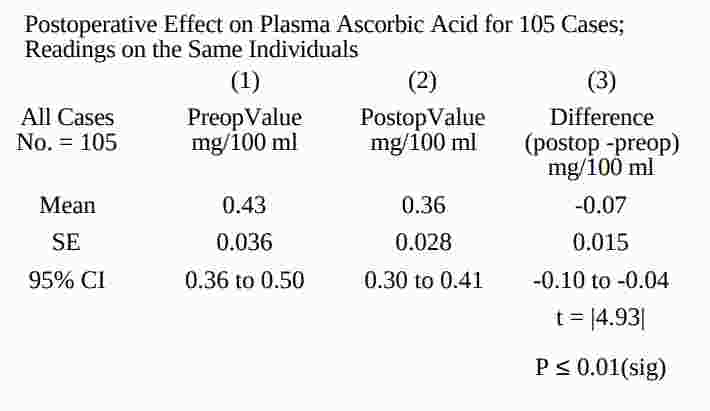
\includegraphics[scale=0.5]{tab3.jpg}
\end{figure}

\begin{enumerate}
\def\labelenumi{\alph{enumi}.}
\tightlist
\item
  \textbf{TRUE (Correct)}
\item
  FALSE
\end{enumerate}

\subsection{Correct rationales}\label{correct-rationales-2}

\begin{itemize}
\tightlist
\item
  The SE in column 3 is the SE for a new variable which is the di
  fference between pre and post and it is different than the SE in
  columns 1 and 2 which correspond to the Se for each individual group.
\item
  You would get contradictory answers since the proper way to calculate
  the standard error for a two-sample t-test is to take the square root
  of the sum of the standard errors of each column. Therefore, the
  correct way is to use the SE's in columns 1 and 2
\end{itemize}

\subsection{Incorrect rationales}\label{incorrect-rationales-2}

\begin{itemize}
\tightlist
\item
  For two-sample test: SE = sqrt (SE1\^{}2 + SE2\^{}2) SE in column3
  comes from SE in columns 1 and 2
\item
  The SE in column 3 is the SE of the sampling distribution of the mean
  difference and 1 and 2 are SE of the respective mean. When computing
  the mean difference, SE calculation accounts for both SEs in 1 and 2.
\end{itemize}

\section{\texorpdfstring{How many calories does a fruit juice popsicle
labeled ``no sugar added'' pack? A random sample of 10 popsicles of a
particular brand is selected, and the calories per serving are measured.
To get a confidence interval for the mean calories per serving of all
no-sugar-added popsicles from this brand, you would
use}{How many calories does a fruit juice popsicle labeled no sugar added pack? A random sample of 10 popsicles of a particular brand is selected, and the calories per serving are measured. To get a confidence interval for the mean calories per serving of all no-sugar-added popsicles from this brand, you would use}}\label{how-many-calories-does-a-fruit-juice-popsicle-labeled-no-sugar-added-pack-a-random-sample-of-10-popsicles-of-a-particular-brand-is-selected-and-the-calories-per-serving-are-measured.-to-get-a-confidence-interval-for-the-mean-calories-per-serving-of-all-no-sugar-added-popsicles-from-this-brand-you-would-use}

\begin{enumerate}
\def\labelenumi{\alph{enumi}.}
\tightlist
\item
  \textbf{the one-sample t interval (Correct)}
\item
  the matched pairs t interval
\item
  the two sample t interval
\item
  the one sample z interval
\end{enumerate}

\subsection{Correct rationales}\label{correct-rationales-3}

\begin{itemize}
\tightlist
\item
  I would use the one-sample t interval because we are only comparing
  one mean and the population standard deviation is unknown.
\end{itemize}

\subsection{Incorrect rationales}\label{incorrect-rationales-3}

\begin{itemize}
\tightlist
\item
  Since we are only inferring about one sample you will do a one sample
  z interval
\end{itemize}

\section{A study is designed to compare the amount of vitamin C (in
milligrams per serving) in oranges that reach the stores either 1 day
after being picked or 3 days after being picked. A random sample of 15
oranges is taken for each group. To test whether there is a difference
in the mean vitamin C amount of all oranges reaching stores either 1 day
or 3 days after being picked, you would
use}\label{a-study-is-designed-to-compare-the-amount-of-vitamin-c-in-milligrams-per-serving-in-oranges-that-reach-the-stores-either-1-day-after-being-picked-or-3-days-after-being-picked.-a-random-sample-of-15-oranges-is-taken-for-each-group.-to-test-whether-there-is-a-difference-in-the-mean-vitamin-c-amount-of-all-oranges-reaching-stores-either-1-day-or-3-days-after-being-picked-you-would-use}

\begin{enumerate}
\def\labelenumi{\alph{enumi}.}
\tightlist
\item
  the one-sample t test
\item
  the one-sample z test
\item
  the one-sample t interval
\item
  the matched pairs t test
\item
  \textbf{the two-sample t test (Correct)}
\end{enumerate}

\subsection{Correct rationales}\label{correct-rationales-4}

\begin{itemize}
\tightlist
\item
  It is a two-sample t test because we are comparing means of two
  different samples. It is not the matched pairs t-test because the two
  samples are not paired, the oranges reaching the stores one day after
  picking do not have an impact on the oranges reaching the stores three
  days after picking, they are independent of each other.
\item
  There are two samples and they are not matched, because the samples
  are not from the same oranges.
\item
  You have two samples, so only D or E should be considered. The way the
  question is worded, we have a random sample for EACH of the groups and
  so it's not a matched test. We measure oranges that get to the store 1
  day after picking and then measure a different group of oranges that
  arrive 3 days after picking.
\end{itemize}

\subsection{Incorrect rationales}\label{incorrect-rationales-4}

\begin{itemize}
\tightlist
\item
  This is a before-after test and so the two samples are not independent
  of each other.
\item
  The matched pairs t test is concerned with the difference between two
  measures in one population. In this case, we wish to compare the mean
  vitamin C amount in the same population (of oranges) at two time
  points post-harvesting: 1 day or 3 days. We are using the t-test
  because the sample size is small (n\textless{}30). Thus we use the
  matched pairs t-test.
\end{itemize}

\section{There are two common methods for measuring the concentration of
a pollutant in fish tissue. Do the results of the two methods differ on
the average? You apply both methods to one sample of 18 carp and
use}\label{there-are-two-common-methods-for-measuring-the-concentration-of-a-pollutant-in-fish-tissue.-do-the-results-of-the-two-methods-differ-on-the-average-you-apply-both-methods-to-one-sample-of-18-carp-and-use}

\begin{enumerate}
\def\labelenumi{\alph{enumi}.}
\tightlist
\item
  \textbf{the one-sample t test (Correct)}
\item
  the one-sample z test
\item
  \textbf{the matched pairs t test (Correct)}
\item
  the two-sample t test
\end{enumerate}

\subsection{Correct rationales}\label{correct-rationales-5}

\begin{itemize}
\tightlist
\item
  A can be correct since can do a t-test on the difference
\item
  This is a matched pairs t test because you are applying the two
  difference methods to the sample sample of fish. Therefore the samples
  are not independent of each other and are paired.
\end{itemize}

\subsection{Incorrect rationales}\label{incorrect-rationales-5}

%\showmatmethods


\bibliography{pinp}
\bibliographystyle{jss}



\end{document}

